\documentclass{beamer}
\usetheme{hpi}

\usepackage{fontspec}
\setmainfont[Path=./beamertheme/]{NeoSans.ttf}

\usepackage[backend=biber]{biblatex}
\bibliography{literature/bibliography.bib}

\usepackage{subcaption}

% These slides also contain speaker notes. You can print just the slides,
% just the notes, or both, depending on the setting below.
% https://github.com/pdfpc/pdfpc
% https://github.com/dannyedel/dspdfviewer
\usepackage{pgfpages}

\setbeameroption{hide notes} % Only slides
%\setbeameroption{show only notes} % Only notes
%\setbeameroption{show notes on second screen=right} % Both

\usepackage{ellipsis} % Leerraumoptimierung
\usepackage{microtype}
\usepackage{booktabs} % Tabellenstriche unterschiedlicher Stärke
\usepackage{tabularx} % Automatische Zeilenumbrüche
\newcolumntype{L}{>{\raggedright\arraybackslash}X}% Linksbündige Spalte ohne Trennung
\newcommand{\ra}[1]{\renewcommand{\arraystretch}{#1}}
\usepackage{minted} % Farbige Hervorhebung von Quellcode
\RequirePackage{csquotes} % Loaded later because of minted
\usepackage{svg}

\title[Multi-Cloud Policies]{Design and Implementation of a Unified Middleware for\\Policy Enforcement in Multi-Cloud Infrastructures}

\date{April 24, 2018}

\author[Jan-Henrich Mattfeld\\Master's Thesis]{Jan-Henrich Mattfeld\texorpdfstring{\\}{, }Master's Thesis}

\institute{Operating Systems and Middleware Group}

\begin{document}

\begin{frame}[title=future_soc_small.jpg]
	\maketitle
\end{frame}


\begin{frame}{Growing Acceptance of Cloud Computing}
\begin{figure}
\centering
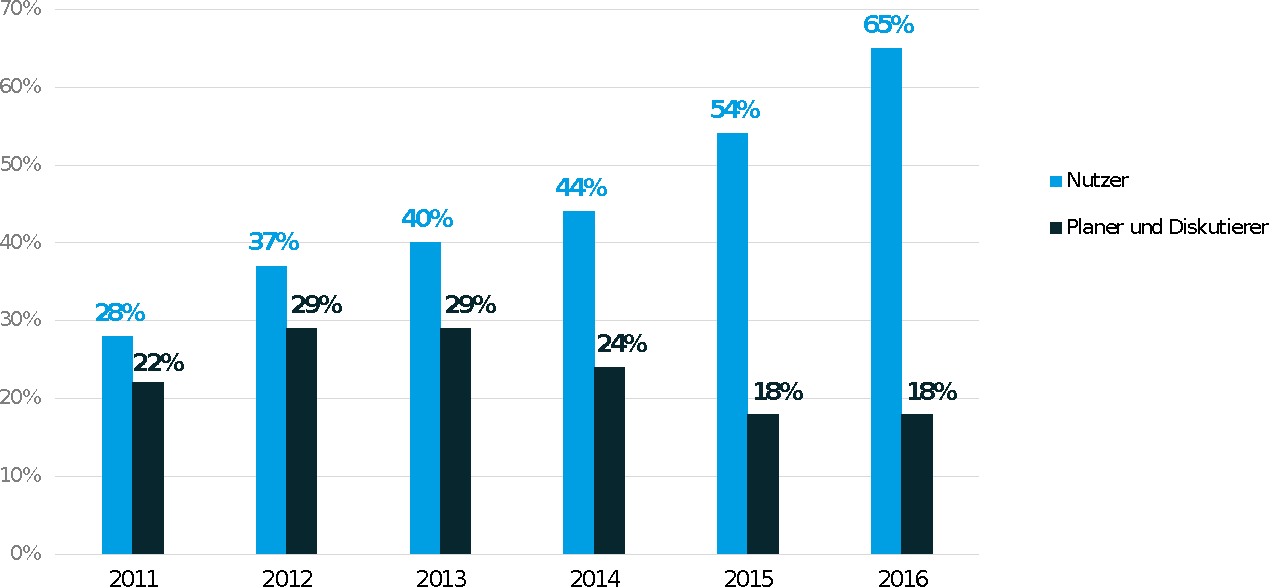
\includegraphics[height=8.5cm]{images/cloud-users.pdf}
\vspace{0.5cm}
\caption{{\tiny Bitkom\,/\,KPMG, \cite{bitkom:2017:cloud-nutzung-unternehmen}}}
\note[item]{Nutzung ist kein Hype, sondern weit Verbreitet.}
\note[item]{Vorteile wie Kosteneinsparungen und Flexibilität}
\note[item]{Aktuelle Zahlen zeigen weiteres Wachstum.}
\end{figure}
\end{frame}


\begin{frame}{Increasing Trust in Cloud Computing}
\begin{figure}
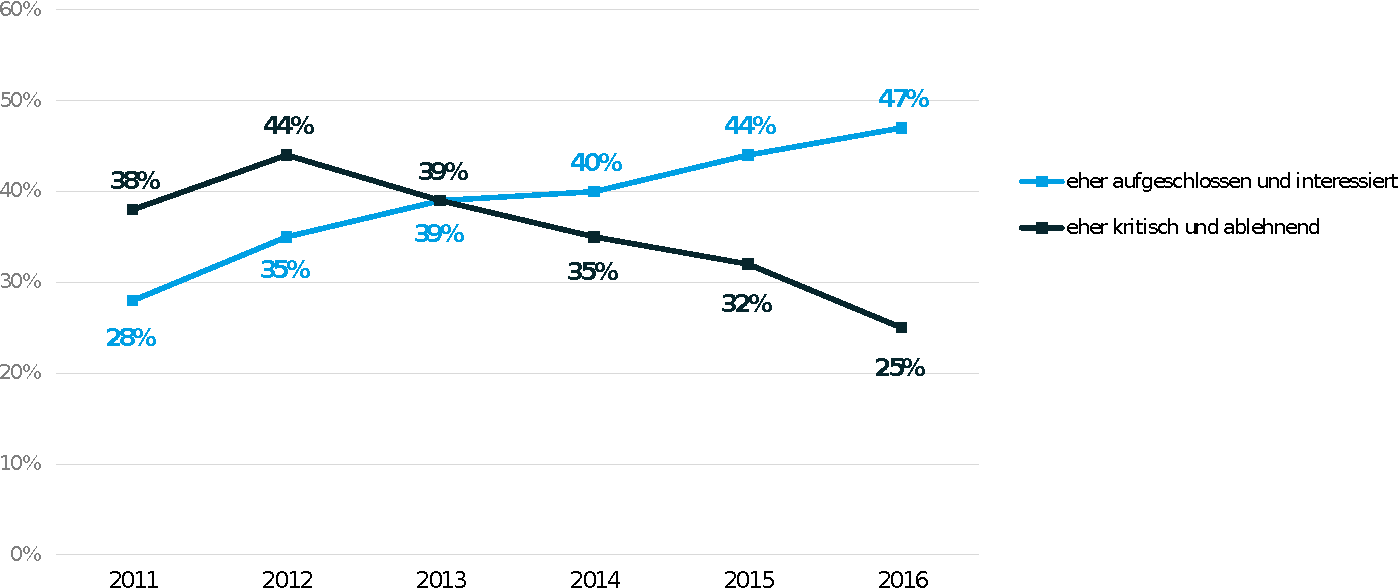
\includegraphics[height=8.5cm]{images/cloud-critics.pdf}
\end{figure}
\note[item]{Vertrauen wächst. Zu Recht?}
\note[item]{McAfee-Studie: Jedes vierte Unternehmen meldet Datendiebstahl in der Cloud}
\end{frame}


\begin{frame}{Actual Trust Issues in Cloud Computing}
\begin{figure}
	\centering
	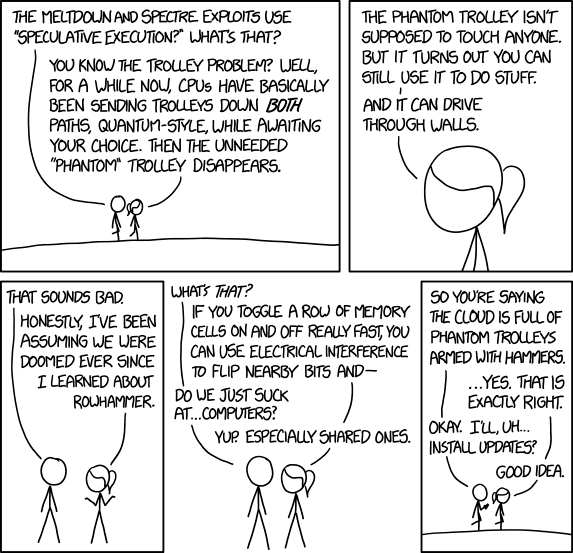
\includegraphics[height=9cm]{images/ideas/xkcd_meltdown_and_spectre.png}
	\caption{{\tiny \url{https://xkcd.com/1938/}}}
	\note[item]{Technische Herausforderungen durch Sicherheitslücken wie Meltdown und Spectre.}
	\note[item]{Durch den ungeschützten Zugriff auf fremde Speicherbereiche war die Mandatentrennung innerhalb virtualisierter Cloud-Umgebungen nicht mehr sichergestellt.}
	\note[item]{Die EU-Datenschutzrichtlinien erfordern sowieso die Speicherung innerhalb bestimmter Regionen.}
	\note[item]{Neues Zugriffsgesetz der USA ist gefährlich.}
	\note[item]{Überwachung und Durchsetzung ist aufwendig.}
\end{figure}
\end{frame}


\begin{frame}{Limited Availability in Cloud Computing}
\begin{figure}
	\centering
	
\includegraphics[height=9cm]{images/ideas/availability-comic.pdf}
	\caption{{\tiny \url{http://turnoff.us/geek/cloud-lock-in/}}}
	\note[item]{Welche Verfügbarkeit bieten die Standard SLAs von Amazon und Microsoft?}
	\note[item]{Azure: 99,95 für virtuelle Maschinen.}
	\note[item]{Bei weniger als 99\% gibt es 25\% Rabatt *wow*}
	\note[item]{Schadensersatz beschränkt sich auf eine Reduzierung der Beiträge.}
\end{figure}
\end{frame}


\begin{frame}{Main Challenges (And a Possible Solution)}
\begin{columns}
\column{0.45\textwidth}
\begin{alertblock}{Data Protection}
	\begin{enumerate}
		\item Regulatory (GDPR)
		\item Technical
	\end{enumerate}	
\end{alertblock}
\note[item]{Wie gerade besprochen.}
\note[item]{Europäisches Datenschutzgesetz}
\pause
\begin{alertblock}{Portability}
	\begin{enumerate}
		\item Data
		\item Applications
	\end{enumerate}
\note[item]{Proprietäre Datenformate}
\note[item]{Cloud-native: Cloud-Provider-spezifisches SDKs}
\end{alertblock}
\column{0.5\textwidth}\pause
\begin{block}{Multi-Cloud-Usage}
Automated with an SLA-aware \newline Cloud Management Platform
\def\svgwidth{\textwidth}
{\tiny \textsf{
\includesvg{./images/multi-cloud-library}}}
\end{block}
\end{columns}
\end{frame}


\begin{frame}{Automation Goals}
\begin{columns}	
	\column{0.45\textwidth}
	\begin{block}<1->{Policies}
		\emph{Event-driven, pre-defined Rules}
		\begin{enumerate}
			\item Restriction of Geo-Locations
			\item Minimum Replication Rate
			\item Storage Encryption
		\end{enumerate}	
	\end{block}
	\note[item]{Einfachste Form.}
	\note[item]{Auch Skalierung: In festgelegt Schritten}
\vspace{1cm}
\begin{block}<3->{Optimization}
	\emph{Optionally, if SLA fulfilled}
	\begin{enumerate}
		\item Use of Sustainable Energy
		\item Pricing
	\end{enumerate}	
	\note[item]{Wenn alle anderen Kriterien erfüllt sind.}
\end{block}
\column{0.45\textwidth}
\begin{block}<2->{SLAs}
\emph{Goal-driven, Dynamic}
\begin{enumerate}
	\item Availability
	\item Throughput
	\item Latency
\end{enumerate}
\note[item]{Strategie flexibel.}
\note[item]{Aufwändiger zu Messen und Umzusetzen.}
\note[item]{Unabhängigkeit von meheren Anbeitern -- wenn Anwendungen portabel.}
\note[item]{Messung für Schadensersatz nötig.}
\note[item]{Überschneidung: Replikation bestimmt auch Verfügbarkeit.}
\end{block}	
\end{columns}
\end{frame}

	

\begin{frame}{SSICLOPS Approach –\\Compact Privacy Policy Language (CPPL) }
\vspace{0.5cm}
\begin{figure}
	\centering
		\def\svgwidth{0.95\textwidth}
	{\tiny \textsf{
			\includesvg{images/ssiclops-cppl}}
	\caption{\cite{ssiclops:d22:intercloud-policies}}}
	\note[item]{CPPL}
	\note[item]{Annotation der Datenpakete (auch Nutzdaten)}
	\note[item]{Cloud-Föderation}
	\note[item]{Provider wissen um ihre Teilnahme und lassen sich beeinflussen.}
\end{figure}
\end{frame}


\begin{frame}{Cloud Broker Research Summary}
\vspace{0.5cm}
\begin{figure}
	\centering
		\def\svgwidth{0.8\textwidth}
	{\tiny \textsf{
	\includesvg{./images/related-work-taxonomy}}}
	\vspace{0.5cm}
	{\tiny \caption{\cite{grozev:2014:cloud-taxonomy}}}
	\note[item]{Kommerzielle Projekte unterstützen nur Policys und keine offenen Standards}
	\note[item]{Forschung setzt auf SLA und Cloud Föderationen.}
	\note[item]{Nicht unbedingt Web-Anwendungen, sondern Batch Jobs}
\end{figure}
\end{frame}


\begin{frame}{Broker Control Cycle}
\begin{figure}
	\def\svgwidth{\textwidth}
	{\tiny \textsf{
			\includesvg{./images/broker-cycle}}}
\end{figure}
\note[item]{Regelkreis erklären.}
\note[item]{Als Inhaltsverzeichnis: SLA-Templates, Anwendungen (Definition und Laufzeitumgebung), Cloud-Connectoren, Brokering-Algorithmus.}
\end{frame}
	

\begin{frame}{Creating Cloud-native Applications}
\begin{figure}
	\centering
	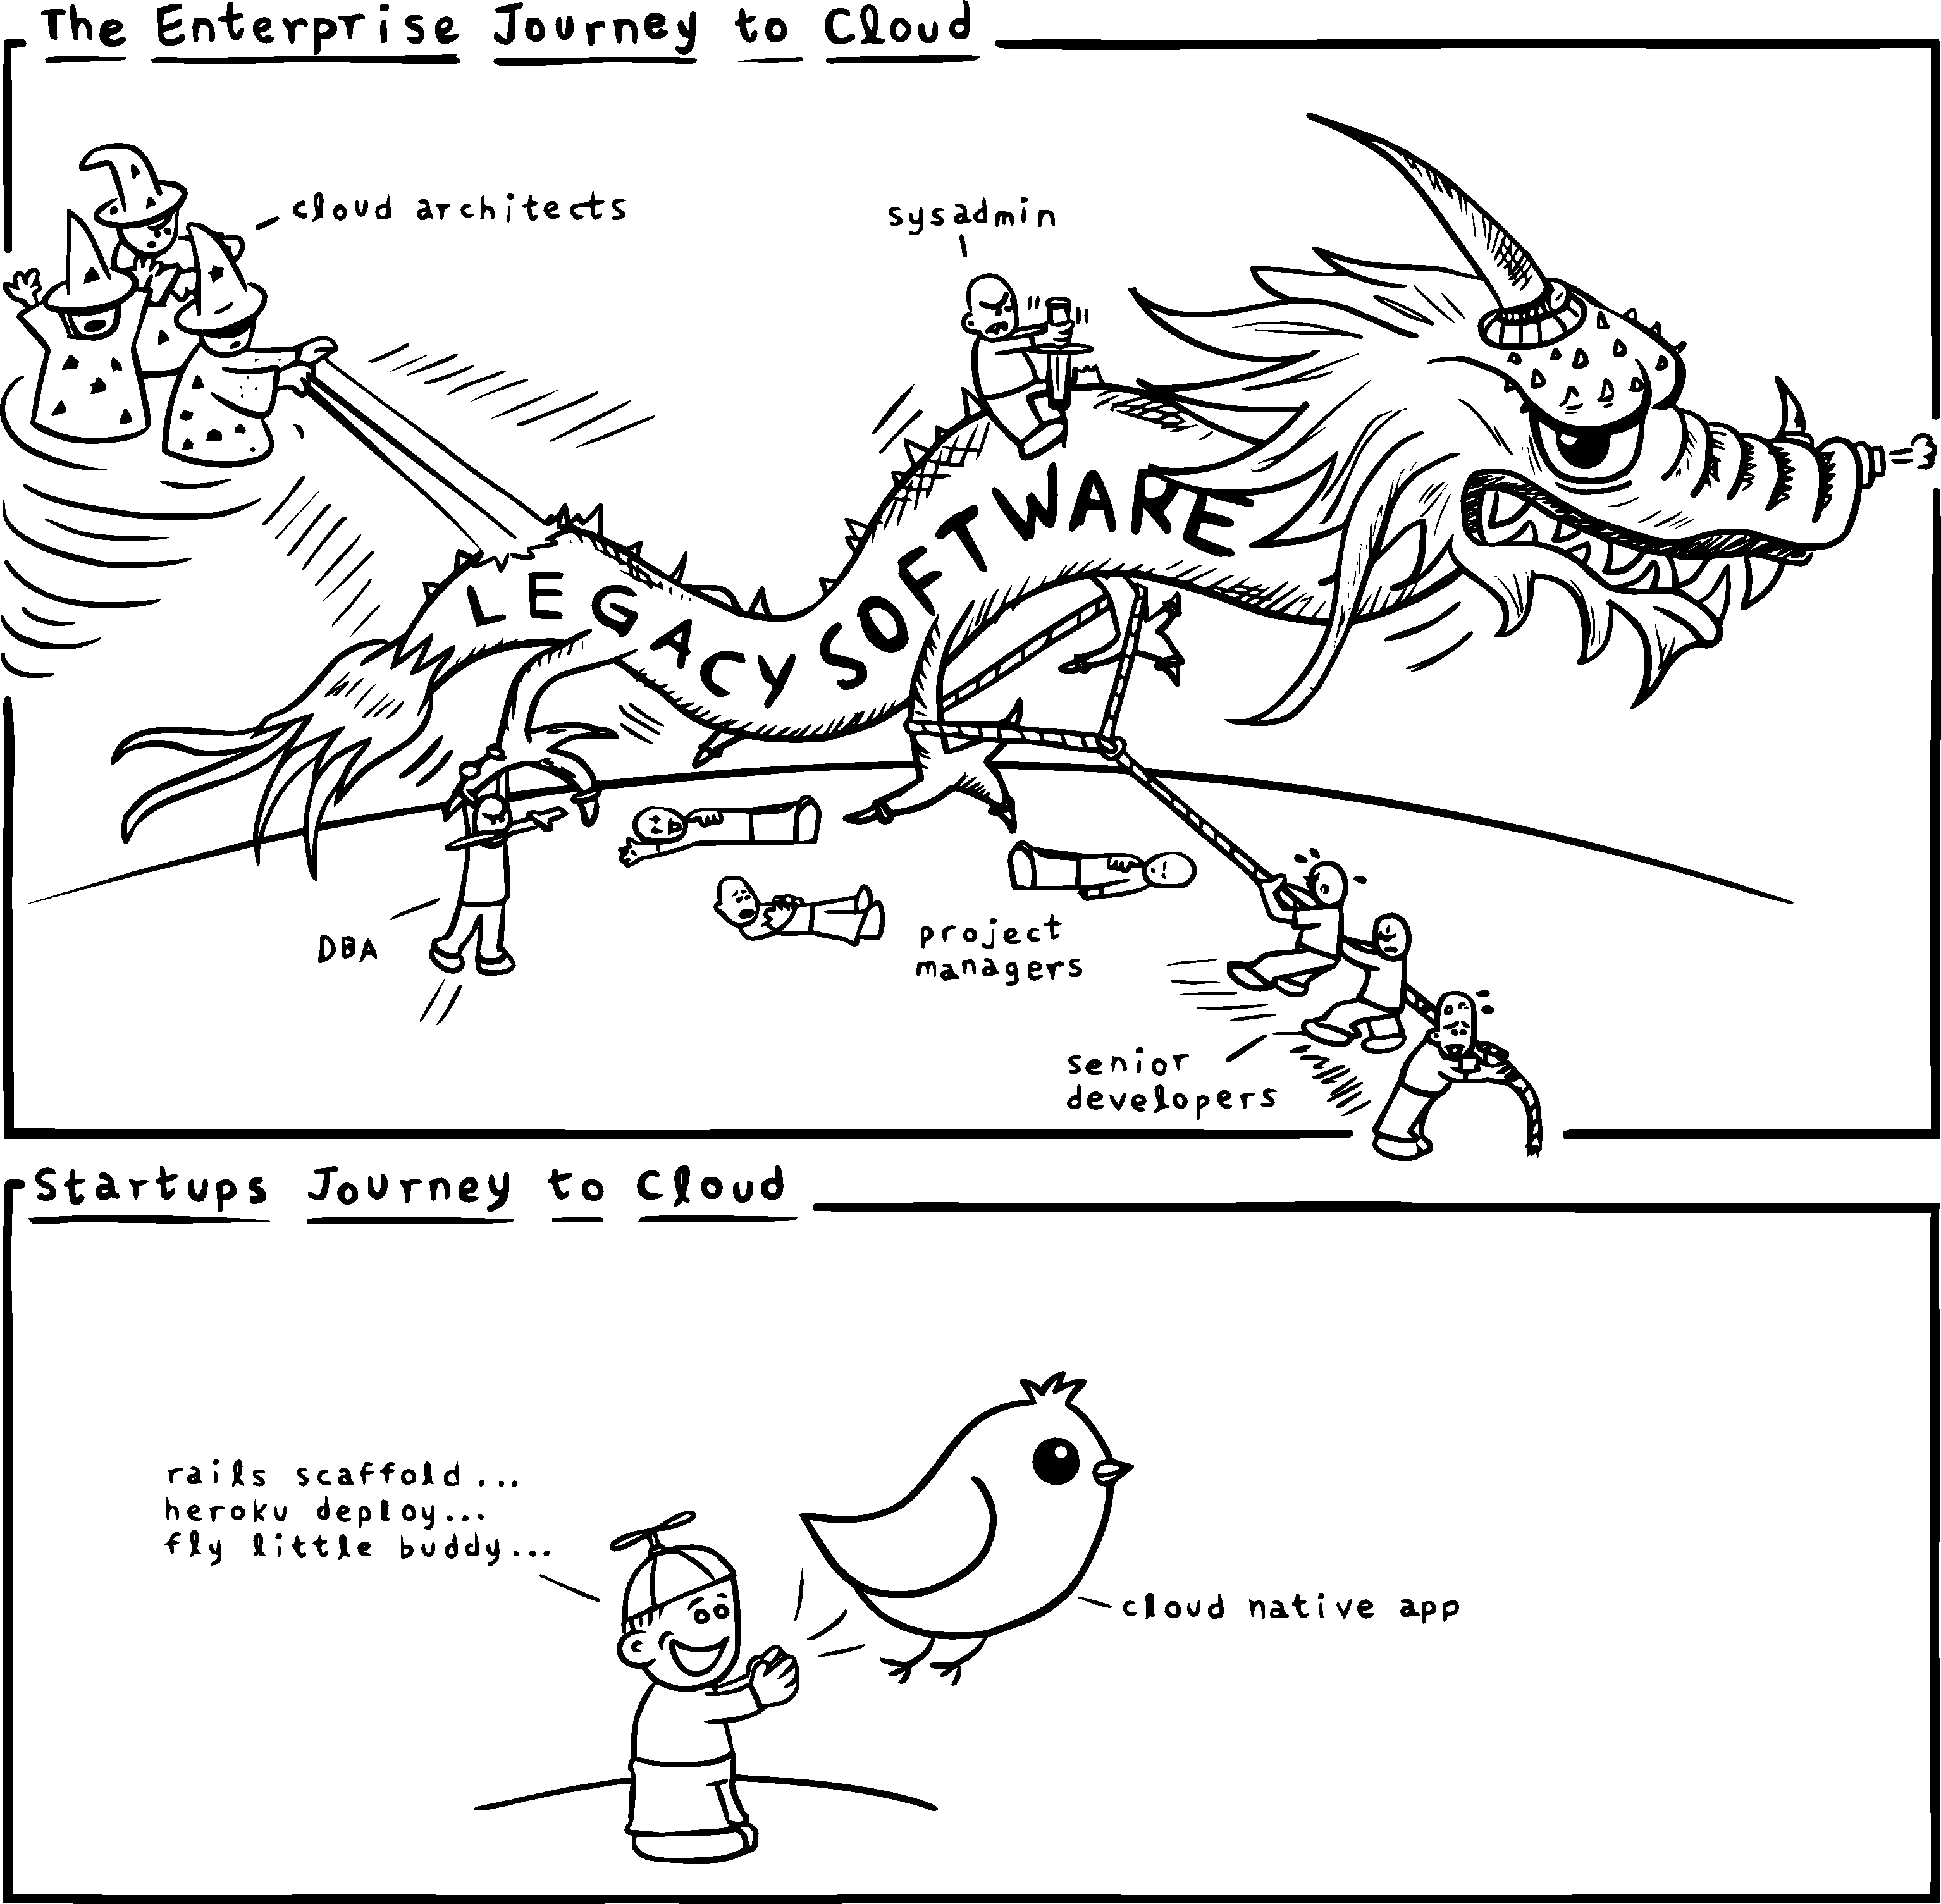
\includegraphics[height=9cm]{images/ideas/enterprise-vs-startup-journey-to-cloud.pdf}
	\caption{{\tiny \url{http://turnoff.us/geek/enterprise-vs-startup-journey-to-cloud/}}}
\end{figure}
\note[item]{Nur zum Teil richtig: Auch bestehende Cloud-native Anwendungen können durch Provider-SDKs unportabel sein.}
\note[item]{Standards nutzen!}
\end{frame}


\begin{frame}{Cloud-ready Runtime Environments}
\vspace{2cm}
\begin{figure}
\begin{subfigure}[b]{0.45\textwidth}		
	\def\svgwidth{\linewidth}
	{\tiny \textsf{
			\includesvg{images/hyrise-r-runtime-vm-wo-text}}}
\end{subfigure}\qquad
\begin{subfigure}[b]{0.45\textwidth}
	\def\svgwidth{\linewidth}
	{\tiny \textsf{
			\includesvg{images/hyrise-r-runtime-docker-wo-text}}}
\end{subfigure}	
\end{figure}
\note[item]{Ubuntu Cloud Images und cloud-init.}
\note[item]{Docker Images und initiale Konfiguration über Docker Entrypoint.}
\note[item]{Konfigurations über Standard Schnittstellen der App.}
\end{frame}
	
	
\begin{frame}{SLA-related Cloud Research (EU)}
	\begin{figure}
		\centering
		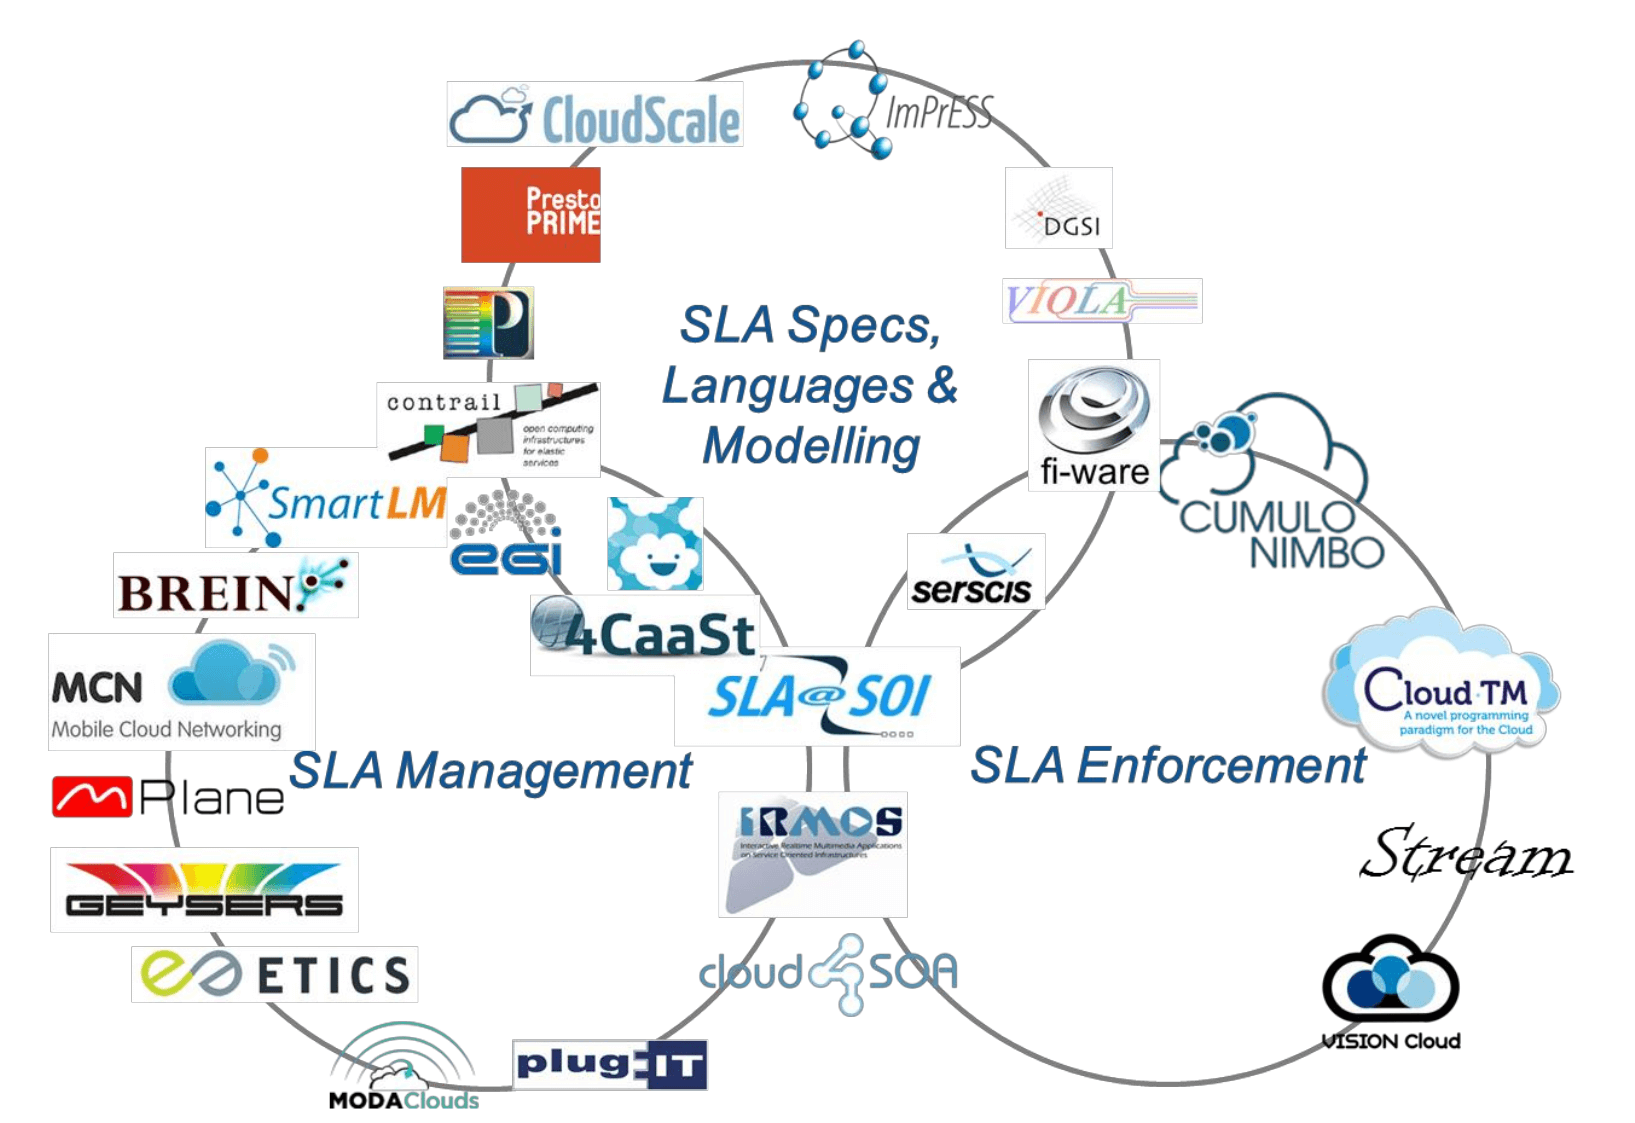
\includegraphics[height=9cm]{images/eu-projects-overview.png}
		\caption{\cite{blasi:2013:eu-projects-overview}}
		\note[item]{Einige verbreitetere Standards: WSDL/SOAP}
		\note[item]{Schwer zu implementieren.}
		\note[item]{Fast jedes Projekt führt eigene SLA-Schemata ein.}
		\note[item]{So kann sich kein Standard durchsetzen.}
		\note[item]{Kommerzielle Anbieter vergrößern die Auswahl noch, ohne offene Standards zu nutzen.}
	\end{figure}
\end{frame}


\begin{frame}[allowframebreaks]{TOSCA –\\Combining Application and SLA}
\inputminted[firstline=15]{yaml}{./src/hyrise-r.sample.yaml}
\note[item]{Topology and Orchestration Specification for Cloud Applications (TOSCA)}
\note[item]{Vereinfacht zu TOSCA-Simple mit YAML}
\end{frame}


\begin{frame}{Broker Implementation}
\begin{figure}
	\def\svgwidth{0.95\textwidth}
	{\tiny \textsf{
			\includesvg{./images/broker-architecture}}}
\end{figure}
\note[item]{Komponentenübergreifender Logger}
\note[item]{Jinja2-Templates (Django)}
\note[item]{Apache Libcloud als Multi-Cloud-Bibliothek.}
\end{frame}

\begin{frame}{Test Application –\\Distributed Research Database Hyrise-R}
\begin{figure}
	\def\svgwidth{0.8\textwidth}
	{\tiny \textsf{
			\includesvg{./images/hyrise-r}}}
	\caption{{\tiny Schwalb et al. \cite{schwalb:2015:hyrise-r}}}
\end{figure}
\end{frame}


\begin{frame}{Hyrise-R Multi-Cloud Testbed}
\begin{figure}
\def\svgwidth{0.8\textwidth}
{\tiny \textsf{
		\includesvg{./images/hyrise-r-deployment}}}
\end{figure}
\end{frame}


\begin{frame}{Test Case I}
\vfill
\begin{table}
	\ra{1.3}%
	\begin{tabularx}{\textwidth}{LLLLL}%
		\toprule%
		%
		Function & Clouds & Policies & SLAs & Optimization\\%
		%
		\midrule%
		%
		Placement & OpenStack, AWS ECS & Geo, Replication & -- & Pricing\\%
	\end{tabularx}
\end{table}
\vfill
\end{frame}


\begin{frame}[fragile]{Placing Algorithm}
\begin{minted}{python}
def place_service(clouds, service_template, sla):
  req_instance_types = service_template.instances
  req_regions = sla.regions

  offered_clouds = filter(c.instance in req_instance_types, clouds)
  offered_regions = filter(c.location in req_regions, offered_clouds)

  offered_prices = sorted(offered_regions, key=k['price'])
  allocated_place = offered_prices[0]

  if allocated_place is None:
    raise SchedulerError("No match. Check resources or change SLA.")
  else:
    return allocated_place
\end{minted}
\end{frame}


\begin{frame}{Test Case II}
\vfill
\begin{table}
\ra{1.3}%
\begin{tabularx}{\textwidth}{LLLLL}%
	\toprule%
	%
	Function & Clouds & Policies & SLAs & Optimization\\%
	%
	\midrule%
	%
	Placement & OpenStack, AWS ECS & Geo, Replication & -- & Pricing\\%
	Scaling   & OpenStack, AWS ECS & Geo, Replication, Workload & Throughput & Pricing\\%
\end{tabularx}
\end{table}
\vfill
\end{frame}


\begin{frame}[fragile]{Scaling Algorithm}
\begin{minted}{python}
def scale(clouds, app_template, sla):
  running_instances = filter_by_app(app_template, clouds)
  idle_instances = filter(has_no_connection(i), running_instances)

  is_replicated = len(running_instances) >= sla.replication_factor
  is_overprovisioned = len(running_instances) >= sla.replication_factor + 1
  meets_throughput = benchmark(app_template, sla) >= sla.throughput
 
  if meets_throughput and is_overprovisioned:
    expensive_idle = sorted(idle_instances, key=i['price'], reverse=True)
    expensive_idle[0].shutdown()
  elif not is_replicated or not meets_throughput:
    place_service(clouds, service_template, sla)
\end{minted}
\end{frame}


\begin{frame}{Results and Outlook I}
	\begin{block}{Unique Combination of Features}
	\begin{enumerate}
		\item Brokering Interactive Web Applications
		\item Multi-Cloud (\emph{Public \& Private})
		\item Multiple Service Models (\emph{IaaS, CaaS})
		\item Policies, SLAs and Optimizations
		\item Metadata-aware (\emph{Geolocation, Pricing})
		\item Built on Open Standards
	\end{enumerate}
\note[item]{Main Contributions}
\note[item]{+ Übersicht Related Work}
\end{block}
\end{frame}


\begin{frame}{Results and Outlook II}
\vspace{2cm}
\begin{columns}
\column{0.45\textwidth}
\begin{alertblock}{Challenges}
	\begin{enumerate}
		\item Variety of Standards and APIs
		\item Libcloud as additional Liability
		\item Operation of Multi-Cloud-Testbeds
	\end{enumerate}
\end{alertblock}
\column{0.45\textwidth}
\pause
\begin{block}{Future Work}
	\begin{enumerate}
		\item Multiple Applications
		\item Dynamically Sized Instances
		\item External Service-Discovery
	\end{enumerate}
\end{block}
\end{columns}
\end{frame}


\begin{frame}{Broker-related Cloud Projects I}
	\ra{1.3}%
	%
	\begin{tabularx}{\textwidth}{LLLLL}%
		%
		\toprule%
		%
		Project or \newline Product & Cloud Architecture & Workload \& Runtimes & Supported Standards & Brokering \& Awareness\\%
		%
		\midrule%
		%
		InterCloud \emph{(Research)} & Centralised Federation & (IaaS, ASP.Net) & Proprietary  & SLA (Geo, Pricing)\\
		%
		Contrail \newline \emph{(EU)} & Centralised Federation & (Hadoop) & Proprietary, OCCI & SLA (Pricing)\\%
		%
		RESERVOIR \newline \emph{(EU)} & Peer-to-peer Federation & Interactive (Java) & OWL, SPARQL & SLA \& Policy (Pricing)\\%
		%
		Optimis \newline \emph{(EU)} & Peer-to-peer Federation & Interactive (IaaS) & Proprietary, OVF & SLA (Pricing)\\%
		%
	\end{tabularx}
\end{frame}


\begin{frame}{Broker-related Cloud Projects II}
\ra{1.3}%
%
\begin{tabularx}{\textwidth}{LLLLL}%
	%
	Bernsetein \emph{(Research)}  & Peer-to-peer Federation & Interactive (IaaS) & Proprietary, XMPP, RDF & SLA (Ress. \& Data Loc.)\\%
	%
	STRATOS \emph{(Research)} & Multi-Cloud & Interactive (IaaS) & Proprietary, SMI  & Policy (Geo, Pricing, Loc.)\\%
	%
	Meryn \emph{(Research)} & Peer-to-peer Federation & (IaaS, Hadoop) & Proprietary  & SLA (Pricing) \\%
	%	
	SeaClouds \newline \emph{(EU)} & Multi-Cloud & Interactive (CF) & TOSCA, CAMP, WS-A & Policy, SLA (App Metrics)\\%
	%
	TOSCAMP \emph{(Research)} & Multi-Cloud & Interactive (IaaS) & TOSCA, CAMP & Policy\\%
	%
\end{tabularx}
\end{frame}


\begin{frame}{Broker-related Cloud Projects III}
	\ra{1.3}%
%
\begin{tabularx}{\textwidth}{LLLLL}%
	%
	Red Hat CloudForms & Multi-Cloud & Interactive (IaaS, CaaS) & Proprietary, Ansible, Heat & Policy\\%
	%
	Rightscale \newline \emph{(CMP)} & Multi-Cloud & Interactive (IaaS, CaaS, PaaS) & Proprietary & Policy (Pricing) \\%
	%
	Scalr \newline \emph{(CMP)} & Multi-Cloud & Interactive (IaaS, CaaS) & Proprietary, Chef, Puppet & Policy (Pricing)\\%
	%
	Cloudify \newline \emph{(CMP)} & Multi-Cloud  & Interactive (IaaS, CaaS)& TOSCA, Puppet & Policy\\%
	%
	\bottomrule%
	%
\end{tabularx}
\end{frame}


\begin{frame}
\frametitle{DevStack Testbed}
\begin{figure}[ht]
	\centering
	\begin{subfigure}[b]{0.45\textwidth}
		\def\svgwidth{\linewidth}
		{\tiny \textsf{
				\includesvg{images/devstack-vm}}}
	\end{subfigure}\qquad
	\begin{subfigure}[b]{0.45\textwidth}
		\def\svgwidth{\linewidth}
		{\tiny \textsf{
				\includesvg{images/devstack-docker}}}
	\end{subfigure}
\end{figure}
\end{frame}


\begin{frame}[allowframebreaks]
\frametitle{References}
\setbeamertemplate{bibliography item}[text]
\printbibliography
\end{frame}


\end{document}
